% !TEX TS-program = XeLaTeX
\documentclass[]{article}
\usepackage[utf8x]{inputenc}
\usepackage{fontspec}
\setmainfont{PragmataPro Mono}
\usepackage[russian]{babel}
\usepackage{hyperref}
\usepackage{amsmath}
\usepackage{amssymb}
\usepackage{cancel}
\usepackage{graphicx}
\usepackage{caption}
\captionsetup{font=small, labelfont=bf, justification=centering}
\graphicspath{ {./pictures/} }
\title{Численные методы}
\author{Александр Голованов}

\begin{document}
\maketitle
\newpage
\tableofcontents
\newpage

\section{18 февраля 2025}
\subsection{Графическое решение нелинейных систем}

\subsubsection{Задача 1}

\begin{gather*}
\begin{cases}
3x-y =-10\\
x^2+y=10
\end{cases}
\end{gather*}

\begingroup
\centering
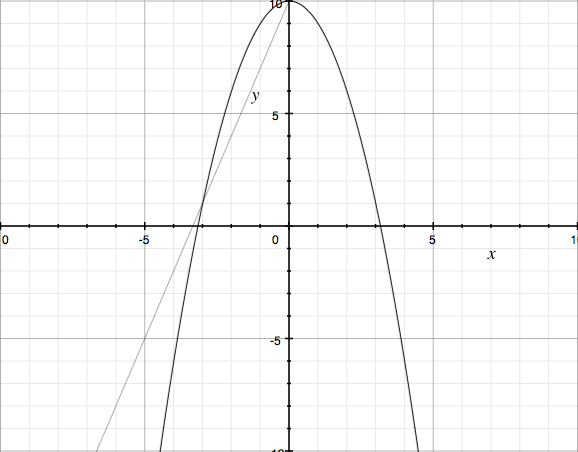
\includegraphics[scale=0.3]{graph1}
\captionof{figure}{Графики задачи 1}
\endgroup

\subsubsection{Задача 2}

\begin{gather*}
\begin{cases}
x-y =5\\
x*y=6
\end{cases}
\end{gather*}

\begingroup
\centering
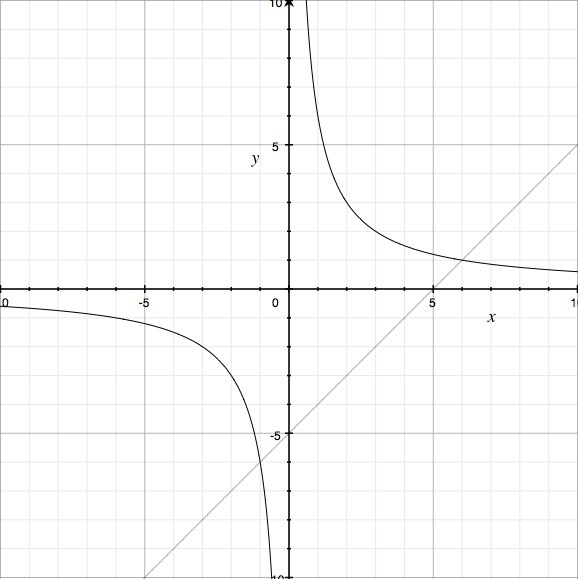
\includegraphics[scale=0.3]{graph2}
\captionof{figure}{Графики задачи 2}
\endgroup

\subsubsection{Задача 3}
\label{ts:task3}
\begin{gather*}
\begin{cases}
x^2+y^2+2xy=9\\
x-y=1
\end{cases}
\end{gather*}

\begingroup
\centering
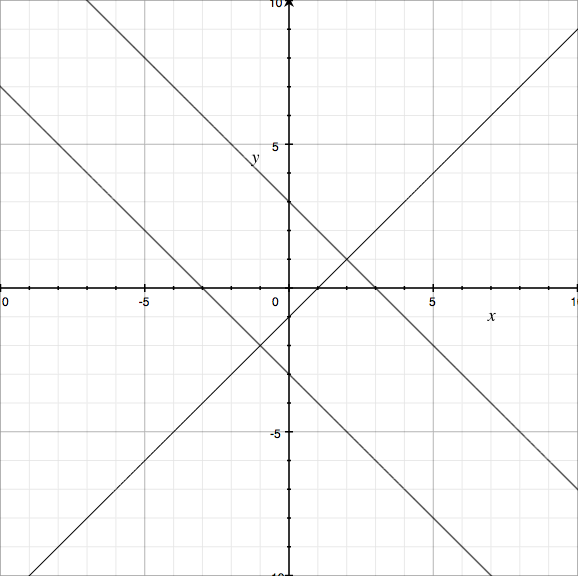
\includegraphics[scale=0.3]{graph3}
\captionof{figure}{Графики задачи 3}
\endgroup
\section{25 февраля 2025}

\subsection{Алгебраические и трансцендентные уравнения}
$g(x) = \phi(x)$
\newline
$x_1 \in X$
\newline
$f(x) = g(x)-\phi(x)=0$
\newline
$g(x)$ и $\phi(x)$ - функции, определенные на некотором промежутке $x$, который называется областью допустимых значений.
\newline
\subsubsection{Задача 4}

\textbf{Условие: } $x^2=2-x$

\begin{gather*}
x^2=2-x\\
x^2+x-2=0\\
x_1 = -1\\
x_2 = -2
\end{gather*}

Решение уравнения - процесс нахождения множества всех его корней или же доказательства их отсутствия. Совокупность нескольких уравнений с несколькими переменными называется системой уравнений. Решение системы уравнений - пара точек, которые при подстановке в каждое уравнение системы дает истинное тождество.
\subsubsection{Задача 5}

\textbf{Условие: }\[
\begin{cases}
x^2+y=5\\
x+y^2=3
\end{cases}
\]

\begingroup
\centering
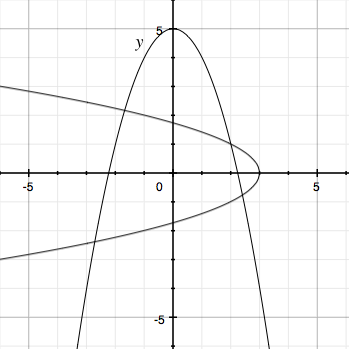
\includegraphics[scale=0.5]{graph4}
\captionof{figure}{Графики задачи 5}
\endgroup



Функция называется алгебраической, если для получения её значения по данному значению $x$ нужно выполнить арифметические действия и возведение в степень с рациональным показателем. Алгебраическая функция называется рациональной относительно $x$, если над. $x$ не производятся другие действия, кроме сложения, вычитания, умножения, деления и возведения в целую степень.
\newline
Типы функций:
\begin{enumerate}
\item Целый: $9x^{15}-4x^{5}+3=0$
\item Дробный: $f(x) = \frac{\sqrt{2}x^2}{8x}$
\item Иррациональный: $f(x)=\sqrt[3]{x+1}+5x^3$
\item Дробно-иррациональный: $\sqrt[4]{\frac{x^3+5x^2+1}{7x^3+4}}+\frac{4x}{3}$
\end{enumerate}

\subsection{Графический метод решения уравнений и систем}

\subsubsection{Задача 6}

\textbf{Условие: } $y=x^3-2x^2+2x-1$
\newline

\begingroup
\centering
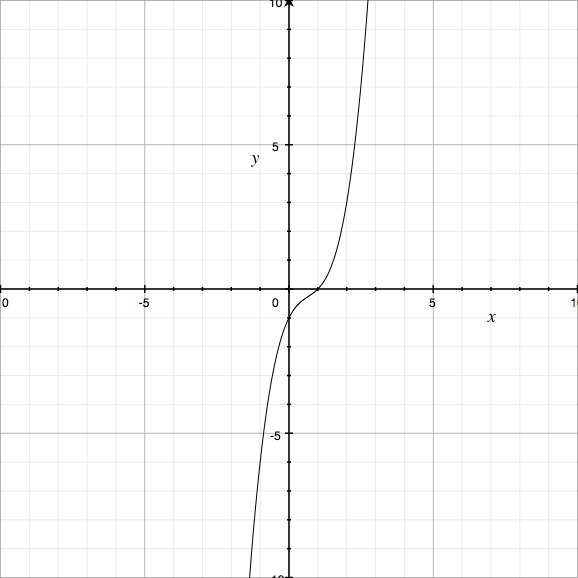
\includegraphics[scale=0.3]{graph5}
\captionof{figure}{Графики задачи 6}
\endgroup

Второй способ: 

\subsubsection{Задача 7}

\textbf{Условие: }$y=x^3-2x^2+2x-1$
\newline

\begingroup
\centering
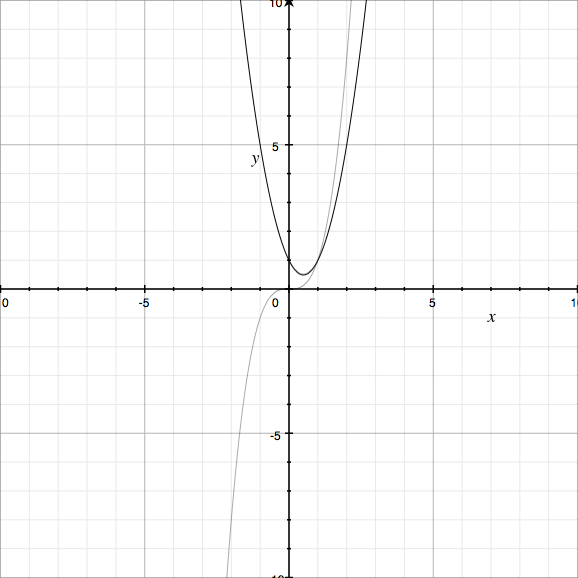
\includegraphics[scale=0.3]{graph6}
\captionof{figure}{Графики задачи 7}
\endgroup

\subsubsection{Задача 8}

\textbf{Условие: } $\lg(x)-3x+5=0$
\newline
\begingroup
\centering
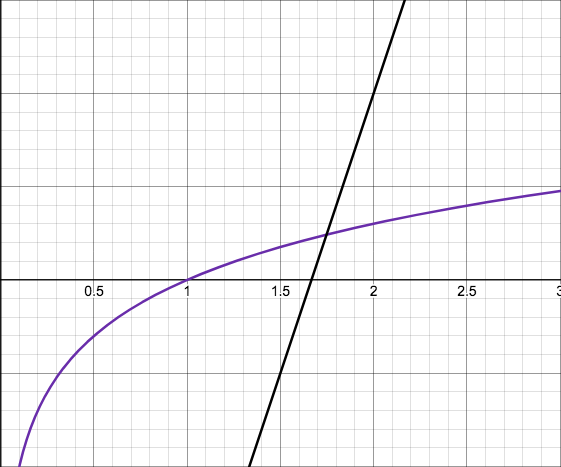
\includegraphics[scale=0.3]{graph7}
\captionof{figure}{Графики задачи 8}
\endgroup

\end{document}